% Capitolul 10: Recapitulare Comprehensivă
% Prezentare academică de calitate Harvard
% Program de licență, Academia de Studii Economice din București

\documentclass[9pt, aspectratio=169, t]{beamer}

% Asigură încadrarea conținutului pe diapozitive
\setbeamersize{text margin left=8mm, text margin right=8mm}

%=============================================================================
% CONFIGURARE TEMĂ ȘI STIL
%=============================================================================
\usetheme{Madrid}
\usecolortheme{seahorse}

% Paletă de Culori Profesională
\definecolor{MainBlue}{RGB}{26, 58, 110}
\definecolor{AccentBlue}{RGB}{42, 82, 140}
\definecolor{IDAred}{RGB}{220, 53, 69}
\definecolor{DarkGray}{RGB}{51, 51, 51}
\definecolor{MediumGray}{RGB}{128, 128, 128}
\definecolor{LightGray}{RGB}{248, 248, 248}
\definecolor{VeryLightGray}{RGB}{235, 235, 235}
\definecolor{Crimson}{RGB}{220, 53, 69}
\definecolor{Forest}{RGB}{46, 125, 50}
\definecolor{Amber}{RGB}{181, 133, 63}
\definecolor{Orange}{RGB}{230, 126, 34}
\definecolor{HarvardCrimson}{RGB}{165, 28, 48}

\setbeamercolor{palette primary}{bg=MainBlue, fg=white}
\setbeamercolor{palette secondary}{bg=MainBlue!85, fg=white}
\setbeamercolor{palette tertiary}{bg=MainBlue!70, fg=white}
\setbeamercolor{structure}{fg=MainBlue}
\setbeamercolor{title}{fg=MainBlue}
\setbeamercolor{frametitle}{fg=MainBlue, bg=white}
\setbeamercolor{block title}{bg=MainBlue, fg=white}
\setbeamercolor{block body}{bg=VeryLightGray, fg=DarkGray}
\setbeamercolor{block title alerted}{bg=Crimson, fg=white}
\setbeamercolor{block body alerted}{bg=Crimson!8, fg=DarkGray}
\setbeamercolor{block title example}{bg=Forest, fg=white}
\setbeamercolor{block body example}{bg=Forest!8, fg=DarkGray}
\setbeamercolor{item}{fg=MainBlue}

\setbeamertemplate{navigation symbols}{}

\setbeamertemplate{footline}{
    \leavevmode%
    \hbox{%
        \begin{beamercolorbox}[wd=.333333\paperwidth,ht=2.5ex,dp=1ex,center]{author in head/foot}%
            \usebeamerfont{author in head/foot}\insertshortauthor
        \end{beamercolorbox}%
        \begin{beamercolorbox}[wd=.333333\paperwidth,ht=2.5ex,dp=1ex,center]{title in head/foot}%
            \usebeamerfont{title in head/foot}\insertshorttitle
        \end{beamercolorbox}%
        \begin{beamercolorbox}[wd=.333333\paperwidth,ht=2.5ex,dp=1ex,right]{date in head/foot}%
            \usebeamerfont{date in head/foot}\insertshortdate{}\hspace*{2em}
            \insertframenumber{} / \inserttotalframenumber\hspace*{2ex}
        \end{beamercolorbox}}%
    \vskip0pt%
}

%=============================================================================
% PACHETE
%=============================================================================
\usepackage[utf8]{inputenc}
\usepackage[T1]{fontenc}
\usepackage{amsmath, amssymb, amsthm}
\usepackage{mathtools}
\usepackage{bm}
\usepackage{tikz}
\usetikzlibrary{arrows.meta, positioning, shapes, calc, decorations.pathreplacing}
\usepackage{booktabs}
\usepackage{multirow}
\usepackage{array}
\usepackage{graphicx}
\usepackage{hyperref}
\usepackage{colortbl}
\hypersetup{colorlinks=false, pdfborder={0 0 0}}
\graphicspath{{../../logos/}{../../charts/}}

%=============================================================================
% MEDII PENTRU TEOREME
%=============================================================================
\theoremstyle{definition}
\setbeamertemplate{theorems}[numbered]
\newtheorem{defn}{Definiție}
\newtheorem{thm}{Teoremă}
\newtheorem{prop}{Propoziție}
\newtheorem{rmk}{Observație}

%=============================================================================
% COMENZI PERSONALIZATE
%=============================================================================
\newcommand{\E}{\mathbb{E}}
\newcommand{\Var}{\text{Var}}
\newcommand{\Cov}{\text{Cov}}
\newcommand{\Corr}{\text{Corr}}
\newcommand{\R}{\mathbb{R}}
\newcommand{\N}{\mathbb{N}}
\newcommand{\Z}{\mathbb{Z}}
\newcommand{\RMSE}{\text{RMSE}}
\newcommand{\MAE}{\text{MAE}}
\newcommand{\MAPE}{\text{MAPE}}

%=============================================================================
% INFORMAȚII TITLU
%=============================================================================
\title[Capitolul 10: Recapitulare]{Capitolul 10: Recapitulare Comprehensivă}
\subtitle{Program de licență, Facultatea de Cibernetică, Statistică și Informatică Economică, Academia de Studii Economice din București}
\author[Prof. dr. Daniel Traian Pele]{Prof. dr. Daniel Traian Pele\\[0.2cm]\footnotesize\texttt{danpele@ase.ro}}
\institute{Academia de Studii Economice din București}
\date{An Universitar 2025--2026}

\begin{document}

%=============================================================================
% DIAPOZITIV TITLU
%=============================================================================
\begin{frame}[plain]
    \begin{tikzpicture}[remember picture, overlay]
        \fill[IDAred] (current page.north west) rectangle ([yshift=-0.15cm]current page.north east);
        \node[anchor=north west] at ([xshift=0.5cm, yshift=-0.3cm]current page.north west) {
            \href{https://www.ase.ro}{\includegraphics[height=1.1cm]{ase_logo.png}}
        };
        \node[anchor=north] at ([yshift=-0.3cm]current page.north) {
            \href{https://ai4efin.ase.ro}{\includegraphics[height=1.1cm]{ai4efin_logo.png}}
        };
        \node[anchor=north east] at ([xshift=-0.5cm, yshift=-0.3cm]current page.north east) {
            \href{https://www.digital-finance-msca.com}{\includegraphics[height=1.1cm]{msca_logo.png}}
        };
    \end{tikzpicture}
    \vfill
    \begin{center}
        {\Large\textcolor{MediumGray}{Analiza și Prognoză Seriilor de Timp}}\\[0.3cm]
        {\Huge\textbf{\textcolor{MainBlue}{Capitolul 10: Recapitulare Completă}}}\\[0.5cm]
        {\Large\textcolor{IDAred}{Studii de Caz Aplicate cu Metodologie Riguroasă}}
    \end{center}
    \vfill

    \begin{tikzpicture}[remember picture, overlay]
        \fill[IDAred] (current page.south west) rectangle ([yshift=0.15cm]current page.south east);
        \node[anchor=south west] at ([xshift=0.5cm, yshift=0.8cm]current page.south west) {
            \href{https://theida.net}{\includegraphics[height=0.9cm]{ida_logo.png}}
        };
        \node[anchor=south] at ([xshift=-3cm, yshift=0.8cm]current page.south) {
            \href{https://blockchain-research-center.com}{\includegraphics[height=0.9cm]{brc_logo.png}}
        };
        \node[anchor=south] at ([yshift=0.8cm]current page.south) {
            \href{https://quantinar.com}{\includegraphics[height=0.9cm]{qr_logo.png}}
        };
        \node[anchor=south] at ([xshift=3cm, yshift=0.8cm]current page.south) {
            \href{https://quantlet.com}{\includegraphics[height=0.9cm]{ql_logo.png}}
        };
        \node[anchor=south east] at ([xshift=-0.5cm, yshift=0.8cm]current page.south east) {
            \href{https://ipe.ro/new}{\includegraphics[height=0.9cm]{acad_logo.png}}
        };
    \end{tikzpicture}
\end{frame}

%=============================================================================
% OUTLINE
%=============================================================================
\begin{frame}{Cuprins}
    \tableofcontents
\end{frame}

%=============================================================================
% SECTION 1: METHODOLOGY
%=============================================================================
\section{Metodologia Prognozei}

\begin{frame}{Abordarea Științifică a Prognozei}
    \begin{block}{Întrebarea de Cercetare}
        Cum putem \textbf{evalua riguros} performanța prognozei evitând supraajustarea?
    \end{block}

    \vspace{0.3cm}

    \begin{alertblock}{Problema Fundamentală}
        \begin{itemize}
            \item Ajustarea în eșantion $\neq$ Performanța în afără eșantionului
            \item Modelele pot ``memora'' datele de antrenament fără a învăța tipare
            \item \textbf{Soluție}: Metodologia corectă train/validation/test
        \end{itemize}
    \end{alertblock}

    \vspace{0.3cm}

    \begin{exampleblock}{Principiu Cheie}
        ``Setul de test trebuie să rămână \textbf{neatins} până la evaluarea finală.'' \\
        \hfill --- Practică standard în machine learning și econometrie
    \end{exampleblock}
\end{frame}

\begin{frame}{Cadrul Train/Validation/Test}
    \begin{center}
        \includegraphics[width=0.9\textwidth]{../charts/train_val_test_split.pdf}
    \end{center}

    \begin{columns}[T]
        \column{0.33\textwidth}
        \begin{block}{Set Antrenament}
            \begin{itemize}
                \item Estimare parametri
                \item Cea mai mare parte
            \end{itemize}
        \end{block}

        \column{0.33\textwidth}
        \begin{block}{Set Validare}
            \begin{itemize}
                \item Comparare modele
                \item Ajustare hiperparam
            \end{itemize}
        \end{block}

        \column{0.33\textwidth}
        \begin{block}{Set Test}
            \begin{itemize}
                \item \textbf{Păstrat}
                \item Metrici finale
            \end{itemize}
        \end{block}
    \end{columns}
\end{frame}

\begin{frame}{Metrici de Evaluare}
    \begin{defn}[Metrici ale Erorii de Prognoză]
        Fie $y_t$ valorile reale, $\hat{y}_t$ prognozele:
        \vspace{-0.2cm}
        \begin{align*}
            \RMSE = \sqrt{\frac{1}{n}\sum_{t}(y_t - \hat{y}_t)^2}, \quad
            \MAE = \frac{1}{n}\sum_{t}|y_t - \hat{y}_t|, \quad
            \MAPE = \frac{100\%}{n}\sum_{t}\left|\frac{y_t - \hat{y}_t}{y_t}\right|
        \end{align*}
    \end{defn}

    \begin{columns}[T]
        \column{0.5\textwidth}
        \begin{exampleblock}{Când să Folosim}
            \begin{itemize}
                \item \textbf{RMSE}: Penalizează erorile mari
                \item \textbf{MAE}: Robust la outlieri
                \item \textbf{MAPE}: Independent de scală (\%)
            \end{itemize}
        \end{exampleblock}

        \column{0.5\textwidth}
        \begin{alertblock}{Atenție}
            \begin{itemize}
                \item MAPE nedefinit când $y_t = 0$
                \item Comparați pe \textbf{același} set test
                \item Raportați metrici \textbf{out-of-sample}
            \end{itemize}
        \end{alertblock}
    \end{columns}
\end{frame}

%=============================================================================
% SECTION 2: BITCOIN VOLATILITY
%=============================================================================
\section{Studiu de Caz 1: Volatilitatea Bitcoin (GARCH)}

\begin{frame}{Bitcoin: Definirea Problemei}
    \begin{block}{Întrebarea de Cercetare}
        Putem prognoză \textbf{volatilitatea} Bitcoin folosind modele GARCH?
    \end{block}

    \vspace{0.2cm}

    \begin{columns}[T]
        \column{0.5\textwidth}
        \textbf{Caracteristicile Datelor}
        \begin{itemize}
            \item Sursă: Yahoo Finance (BTC-USD)
            \item Perioadă: Ian 2019 -- Ian 2025
            \item Frecvență: Zilnică
            \item Observații: $\approx 2.200$ zile
        \end{itemize}

        \vspace{0.3cm}

        \textbf{Fapte Stilizate}
        \begin{itemize}
            \item Randamente: medie aproape zero
            \item Cozi groase (curtosis $> 3$)
            \item Clustering al volatilității
        \end{itemize}

        \column{0.5\textwidth}
        \begin{alertblock}{Insight Cheie}
            Randamentele financiare sunt de obicei:
            \begin{itemize}
                \item \textbf{Impredictibile} în medie
                \item \textbf{Predictibile} în varianță
            \end{itemize}

            \vspace{0.2cm}
            $\Rightarrow$ Focus pe \textbf{prognoză volatilității}
        \end{alertblock}
    \end{columns}
\end{frame}

\begin{frame}{Bitcoin: Clustering-ul Volatilității}
    \begin{center}
        \includegraphics[width=0.88\textwidth]{../charts/btc_returns.pdf}
    \end{center}

    \begin{exampleblock}{Observație}
        Randamentele mari tind să urmeze randamente mari, cele mici urmează cele mici. Acesta este \textbf{clustering-ul volatilității}---fenomenul pe care GARCH îl captează.
    \end{exampleblock}
\end{frame}

\begin{frame}{Bitcoin: Dovezi pentru GARCH}
    \begin{columns}[T]
        \column{0.5\textwidth}
        \begin{center}
            \includegraphics[width=\textwidth]{../charts/btc_squared_returns.pdf}
        \end{center}
        \vspace{0.1cm}
        {\small Randamentele pătrate $r_t^2$ sunt proxy pentru volatilitate $\sigma_t^2$. Vârfurile se grupează.}

        \column{0.5\textwidth}
        \begin{center}
            \includegraphics[width=\textwidth]{../charts/btc_acf_squared.pdf}
        \end{center}
        \vspace{0.1cm}
        {\small Barele ACF depășesc benzile albastre $\Rightarrow$ autocorelație semnificativă.}
    \end{columns}

    \vspace{0.2cm}

    \begin{alertblock}{De ce GARCH?}
        Dacă $r_t^2$ ar fi zgomot alb, ACF ar fi zero. ACF semnificativ înseamnă că \textbf{volatilitatea trecută prezice volatilitatea viitoare}---GARCH captează asta!
    \end{alertblock}
\end{frame}

\begin{frame}{Specificarea Modelului GARCH}
    \begin{defn}[Modelul GARCH(p,q)]
        Fie $r_t$ randamentele. Modelul GARCH(p,q) este:
        \begin{align*}
            r_t &= \mu + \varepsilon_t, \quad \varepsilon_t = \sigma_t z_t, \quad z_t \sim N(0,1) \\[0.2cm]
            \sigma_t^2 &= \omega + \sum_{i=1}^{q}\alpha_i \varepsilon_{t-i}^2 + \sum_{j=1}^{p}\beta_j \sigma_{t-j}^2
        \end{align*}
        unde $\omega > 0$, $\alpha_i \geq 0$, $\beta_j \geq 0$, și $\sum_{i=1}^{q}\alpha_i + \sum_{j=1}^{p}\beta_j < 1$.
    \end{defn}

    \vspace{0.3cm}

    \begin{columns}[T]
        \column{0.5\textwidth}
        \begin{block}{Variante de Model}
            \begin{itemize}
                \item \textbf{GARCH(1,1)}: Cel mai comun
                \item \textbf{GJR-GARCH}: Efect de levier
                \item \textbf{EGARCH}: Șocuri asimetrice
            \end{itemize}
        \end{block}

        \column{0.5\textwidth}
        \begin{exampleblock}{Interpretare}
            \begin{itemize}
                \item $\alpha$: Impactul șocurilor trecute
                \item $\beta$: Persistența volatilității
                \item $\alpha + \beta \approx 1$: Persistență înaltă
            \end{itemize}
        \end{exampleblock}
    \end{columns}
\end{frame}

\begin{frame}{Bitcoin: Împărțirea Datelor și Staționaritate}
    \begin{columns}[T]
        \column{0.5\textwidth}
        \begin{block}{Împărțirea Datelor}
            \begin{center}
            \begin{tabular}{lrr}
                \toprule
                \textbf{Set} & \textbf{Perioadă} & \textbf{N} \\
                \midrule
                Antrenament (70\%) & 2019-01 -- 2023-03 & 1.543 \\
                Validare (20\%) & 2023-03 -- 2024-06 & 441 \\
                Test (10\%) & 2024-06 -- 2025-01 & 221 \\
                \midrule
                \textbf{Total} & & \textbf{2.205} \\
                \bottomrule
            \end{tabular}
            \end{center}
        \end{block}

        \column{0.5\textwidth}
        \begin{block}{Teste de Staționaritate}
            \begin{center}
            \begin{tabular}{lcc}
                \toprule
                \textbf{Serie} & \textbf{ADF} & \textbf{Rezultat} \\
                \midrule
                Prețuri & $p = 0.50$ & Non-staționară \\
                Randamente & $p < 0.01$ & \textcolor{Forest}{Staționară} \\
                \bottomrule
            \end{tabular}
            \end{center}

            \vspace{0.3cm}

            $\Rightarrow$ Modelăm \textbf{randamente}, nu prețuri
        \end{block}
    \end{columns}

    \vspace{0.3cm}

    \begin{alertblock}{De ce Contează Staționaritatea}
        GARCH necesită input slab staționar. Prețurile urmează random walk; randamentele sunt staționare.
    \end{alertblock}
\end{frame}

\begin{frame}{Bitcoin: Selectarea Modelului pe Setul de Validare}
    \begin{block}{Metodologie}
        Eștimăm fiecare model pe \textbf{datele de antrenament}, evaluăm pe \textbf{setul de validare}.
    \end{block}

    \vspace{0.3cm}

    \begin{center}
    \begin{tabular}{lcccl}
        \toprule
        \textbf{Model} & \textbf{AIC} & \textbf{BIC} & \textbf{Val MAE} & \textbf{Selectare} \\
        \midrule
        GARCH(1,1) & 6.994,8 & 7.020,6 & \textbf{2,638} & \cellcolor{Forest!20}\textbf{Cel mai bun} \\
        GARCH(2,1) & 6.993,7 & 7.024,6 & 2,640 & \\
        GJR-GARCH(1,1) & 6.983,7 & 7.014,6 & 2,669 & \\
        EGARCH(1,1) & --- & --- & --- & Eșuat$^*$ \\
        \bottomrule
    \end{tabular}
    \end{center}

    \vspace{0.1cm}
    {\footnotesize $^*$Prognoze analitice indisponibile pentru $h > 1$}

    \vspace{0.3cm}

    \begin{exampleblock}{Rezultat}
        \textbf{GARCH(1,1)} selectat pe baza celui mai mic MAE de validare pentru prognozele de volatilitate.
    \end{exampleblock}
\end{frame}

\begin{frame}{Bitcoin: Evaluarea Finală pe Setul de Test}
    \begin{center}
        \includegraphics[width=0.68\textwidth]{../charts/garch_forecast.pdf}
    \end{center}
    \vspace{-0.1cm}
    \begin{columns}[T]
        \column{0.5\textwidth}
        \begin{block}{Parametri}
            $\omega=0,87$, $\alpha=0,09$, $\beta=0,84$\\
            $\alpha + \beta = 0,93$ (persistență înaltă)
        \end{block}

        \column{0.5\textwidth}
        \begin{exampleblock}{Performanță Test}
            MAE = 1,82, RMSE = 2,14\\
            Prognoză urmărește bine volatilitatea realizată.
        \end{exampleblock}
    \end{columns}
\end{frame}

\begin{frame}{GARCH: Prognozele Multi-Step Converg}
    \begin{center}
        \includegraphics[width=0.65\textwidth]{../charts/garch_convergence.pdf}
    \end{center}

    \begin{exampleblock}{Insight Cheie}
        Prognozele multi-step converg la $\bar{\sigma}^2 = \frac{\omega}{1-\alpha-\beta}$. Soluția: prognoze rolling one-step-ahead.
    \end{exampleblock}
\end{frame}

\begin{frame}{GARCH: Soluția Rolling One-Step-Ahead}
    \begin{center}
        \includegraphics[width=0.85\textwidth]{../charts/rolling_vs_multistep.pdf}
    \end{center}

    \begin{columns}[T]
        \column{0.5\textwidth}
        \begin{block}{Multi-Step (Stânga)}
            Converge la $\bar{\sigma}^2$ \textcolor{Crimson}{(plat)}
        \end{block}

        \column{0.5\textwidth}
        \begin{exampleblock}{Rolling 1-Step (Dreapta)}
            Re-estimare la fiecare $t$ \textcolor{Forest}{(dinamic)}
        \end{exampleblock}
    \end{columns}
\end{frame}

\begin{frame}{Bitcoin: Prognoză Volatilității GARCH (Set Test)}
    \begin{center}
        \includegraphics[width=0.72\textwidth]{../charts/garch_forecast.pdf}
    \end{center}
    \vspace{-0.15cm}
    \begin{exampleblock}{Rezultat}
        Prognozele rolling one-step-ahead GARCH(1,1) captează \textbf{tiparele dinamice ale volatilității}. Linia roșie urmărește volatilitatea realizată (zona albastră).
    \end{exampleblock}
\end{frame}

\begin{frame}{Bitcoin: Concluzii Cheie}
    \begin{columns}[T]
        \column{0.6\textwidth}
        \begin{block}{Sumar}
            \begin{enumerate}
                \item \textbf{Randamentele sunt staționare}; prețurile nu
                \item \textbf{GARCH(1,1)} depășește variantele mai complexe
                \item \textbf{Persistență înaltă} ($\alpha + \beta = 0,93$)
                \item Volatilitatea este \textbf{predictibilă} chiar când randamentele nu sunt
            \end{enumerate}
        \end{block}

        \vspace{0.3cm}

        \begin{exampleblock}{Implicații Practice}
            \begin{itemize}
                \item Managementul riscului: VaR, Expected Shortfall
                \item Evaluarea opțiunilor necesită prognoze de volatilitate
                \item Optimizarea portofoliului cu risc variabil în timp
            \end{itemize}
        \end{exampleblock}

        \column{0.4\textwidth}
        \begin{alertblock}{Limitări}
            \begin{itemize}
                \item GARCH presupune șocuri \textbf{simetrice}
                \item Nu captează \textbf{salturi}
                \item Distribuția normală poate fi restrictivă
            \end{itemize}
        \end{alertblock}

        \vspace{0.3cm}

        \begin{block}{Extensii}
            \begin{itemize}
                \item Inovații Student-t
                \item Volatilitate realizată
                \item Modele HAR
            \end{itemize}
        \end{block}
    \end{columns}
\end{frame}

\begin{frame}{Bitcoin: Fapte Stilizate GARCH}
    \begin{columns}[T]
        \column{0.5\textwidth}
        \begin{center}
            \includegraphics[width=\textwidth]{../charts/btc_squared_returns.pdf}
        \end{center}
        {\small Randamente pătrate $r_t^2$ ca proxy pentru volatilitate. Observați clustering-ul perioadelor de volatilitate înaltă.}

        \column{0.5\textwidth}
        \begin{block}{Fapte Stilizate Financiare}
            \begin{enumerate}
                \item \textbf{Clustering volatilitate}: Mișcări mari urmează mișcări mari
                \item \textbf{Cozi groase}: Mai multe evenimente extreme decât prezice Normala
                \item \textbf{Efect leverage}: Randamente negative $\succ$ volatilitate mai mare
                \item \textbf{Reversie la medie}: Volatilitatea revine la nivelul pe termen lung
            \end{enumerate}
        \end{block}
    \end{columns}

    \vspace{0.2cm}

    \begin{alertblock}{De Ce Funcționează GARCH}
        GARCH captează faptele 1 \& 4. Pentru faptul 3, folosiți GJR-GARCH sau EGARCH. Pentru faptul 2, folosiți inovații Student-t.
    \end{alertblock}
\end{frame}

%=============================================================================
% SECTION 3: SUNSPOTS
%=============================================================================
\section{Studiu de Caz 2: Ciclurile Petelor Solare (Fourier)}

\begin{frame}{Pete Solare: Ciclul Solar de 11 Ani}
    \begin{columns}[T]
        \column{0.55\textwidth}
        \begin{center}
            \includegraphics[width=\textwidth]{../charts/sunspots.pdf}
        \end{center}
        {\small Liniile punctate marchează vârfurile ciclului ($\approx$ la fiecare 11 ani). Amplitudinea variază.}

        \column{0.45\textwidth}
        \begin{center}
            \includegraphics[width=\textwidth]{../charts/sunspots_acf.pdf}
        \end{center}
        {\small ACF are vârfuri la lag 11 și 22, confirmând periodicitatea ciclului solar.}
    \end{columns}

    \vspace{0.2cm}

    \begin{alertblock}{Provocare}
        SARIMA$(p,d,q)(P,D,Q)_{11}$ necesită estimarea lag-urilor sezoniere la 11, 22, 33... Prea mulți parametri! \textbf{Soluție}: Termeni Fourier.
    \end{alertblock}
\end{frame}

\begin{frame}{Termeni Fourier pentru Sezonalitate}
    \begin{center}
        \includegraphics[width=0.85\textwidth]{../charts/fourier_terms.pdf}
    \end{center}

    \begin{columns}[T]
        \column{0.55\textwidth}
        \begin{block}{Cum Funcționează}
            Aproximăm orice tipar periodic folosind unde sinus și cosinus:
            $S_t = \sum_{k=1}^{K}\left[\alpha_k \sin\left(\frac{2\pi k t}{s}\right) + \beta_k \cos\left(\frac{2\pi k t}{s}\right)\right]$
        \end{block}

        \column{0.45\textwidth}
        \begin{exampleblock}{Insight Cheie}
            \begin{itemize}
                \item $K=1$: Undă simplă (2 param)
                \item $K=3$: Formă complexă (6 param)
                \item Pete solare: $s=11$, $K=3$
            \end{itemize}
        \end{exampleblock}
    \end{columns}
\end{frame}

\begin{frame}{Pete Solare: Selectarea Modelului}
    \begin{block}{Metodologie}
        Comparăm $K = 1, 2, 3, 4$ armonici Fourier pe setul de validare.
    \end{block}

    \vspace{0.2cm}

    \begin{columns}[T]
        \column{0.5\textwidth}
        \begin{center}
        \textbf{Împărțirea Datelor}
        \begin{tabular}{lrr}
            \toprule
            \textbf{Set} & \textbf{Perioadă} & \textbf{N} \\
            \midrule
            Antrenament (70\%) & 1900--1975 & 76 \\
            Validare (20\%) & 1976--1997 & 22 \\
            Test (10\%) & 1998--2008 & 11 \\
            \midrule
            \textbf{Total} & & \textbf{109} \\
            \bottomrule
        \end{tabular}
        \end{center}

        \column{0.5\textwidth}
        \begin{center}
        \textbf{Comparație Modele}
        \begin{tabular}{cccc}
            \toprule
            \textbf{K} & \textbf{AIC} & \textbf{Val RMSE} & \\
            \midrule
            1 & 665,9 & 87,15 & \\
            2 & 668,0 & 86,92 & \\
            \rowcolor{Forest!20} 3 & 671,8 & \textbf{86,81} & Cel mai bun \\
            4 & 674,5 & 87,93 & \\
            \bottomrule
        \end{tabular}
        \end{center}
    \end{columns}

    \vspace{0.3cm}

    \begin{exampleblock}{Rezultat}
        \textbf{K = 3} armonici Fourier selectate (6 parametri pentru ciclul de 11 ani).
    \end{exampleblock}
\end{frame}

\begin{frame}{Pete Solare: Rezultate Prognoză}
    \begin{center}
        \includegraphics[width=0.75\textwidth]{../charts/sunspot_forecast.pdf}
    \end{center}
    \vspace{-0.15cm}
    \begin{columns}[T]
        \column{0.5\textwidth}
        \begin{block}{Model}
            ARIMA(2,0,1) + 3 termeni Fourier captează dinamică ciclului de 11 ani.
        \end{block}

        \column{0.5\textwidth}
        \begin{exampleblock}{Performanță Test}
            RMSE = 31,10, MAE = 25,83. Modelul urmărește tiparul general al ciclului.
        \end{exampleblock}
    \end{columns}
\end{frame}

\begin{frame}{Pete Solare: Concluzii Cheie}
    \begin{columns}[T]
        \column{0.5\textwidth}
        \begin{block}{Când să Folosiți Termeni Fourier}
            \begin{itemize}
                \item Perioada sezonieră $s$ este \textbf{lungă} (ex: 11 ani, 52 săptămâni)
                \item SARIMA ar necesită prea multe lag-uri sezoniere
                \item Tiparul este \textbf{neted și periodic}
                \item Trebuie capturate cicluri multiple
            \end{itemize}
        \end{block}

        \vspace{0.2cm}

        \begin{alertblock}{Alegerea lui K}
            Începeți cu $K=1$, creșteți până când eroarea de validare nu mai scade. K prea mare = supraajustare.
        \end{alertblock}

        \column{0.5\textwidth}
        \begin{exampleblock}{Fourier vs SARIMA}
            \begin{center}
            \begin{tabular}{lcc}
                \toprule
                & \textbf{Fourier} & \textbf{SARIMA} \\
                \midrule
                Sezoane lungi & \checkmark & $\times$ \\
                Sezoane scurte & OK & \checkmark \\
                Parametri & $2K$ & Mulți \\
                Flexibilitate & Fixă & Adaptivă \\
                \bottomrule
            \end{tabular}
            \end{center}
        \end{exampleblock}

        \vspace{0.2cm}

        \begin{block}{Aplicații}
            Cicluri climatice, cicluri de afaceri, fenomene astronomice
        \end{block}
    \end{columns}
\end{frame}

%=============================================================================
% SECTION 4: UNEMPLOYMENT
%=============================================================================
\section{Studiu de Caz 3: Șomajul (Prophet)}

\begin{frame}{Șomajul: Train / Validation / Test Split}
    \begin{center}
        \includegraphics[width=0.85\textwidth]{../charts/unemployment_train_val_test.pdf}
    \end{center}
    \vspace{-0.1cm}
    \begin{block}{Metodologie}
        \textbf{Training} (70\%): Estimare modele. \textbf{Validare} (20\%): Selecție model. \textbf{Test} (10\%): Evaluare finală.
    \end{block}
\end{frame}

\begin{frame}{Șomajul: Analiză Preliminără}
    \begin{center}
        \includegraphics[width=0.82\textwidth]{../charts/unemployment_acf_pacf.pdf}
    \end{center}

    \begin{columns}[T]
        \column{0.5\textwidth}
        \begin{block}{Interpretare ACF}
            Descreștere lentă $\Rightarrow$ serie nestaționară. Necesită diferențiere ($d \geq 1$).
        \end{block}

        \column{0.5\textwidth}
        \begin{exampleblock}{Interpretare PACF}
            Vârf semnificativ la lag 1 sugerează componentă AR(1). Pattern sezonier la lag 12.
        \end{exampleblock}
    \end{columns}
\end{frame}

\begin{frame}{Șomajul: Teste de Staționaritate}
    \begin{center}
        \includegraphics[width=0.68\textwidth]{../charts/unemployment_stationarity.pdf}
    \end{center}

    \begin{columns}[T]
        \column{0.5\textwidth}
        \begin{alertblock}{Original: ADF p = 0,056}
            Nestaționară (ACF descreștere lentă)
        \end{alertblock}

        \column{0.5\textwidth}
        \begin{exampleblock}{Diferențiată: ADF p $<$ 0,001}
            Staționară $\Rightarrow$ folosim $d=1$
        \end{exampleblock}
    \end{columns}
\end{frame}

\begin{frame}{Șomajul: Selecția Modelului (Set Validare)}
    \begin{center}
        \includegraphics[width=0.78\textwidth]{../charts/sarima_model_selection.pdf}
    \end{center}
    \vspace{-0.2cm}
    \begin{block}{Best: SARIMA(1,1,1)(1,0,0)$_{12}$}
        Fit pe training (70\%), evaluare pe validare (20\%). Cel mai bun model selectat după Val RMSE minim.
    \end{block}
\end{frame}

\begin{frame}{Șomajul: Parametrii SARIMA}
    \begin{center}
        \includegraphics[width=0.65\textwidth]{../charts/sarima_parameters.pdf}
    \end{center}

    \begin{block}{SARIMA(1,1,1)(1,0,0)$_{12}$ eștimat pe Train+Val (2010-2019)}
        AR(1): $\phi_1 = -0,86$, MA(1): $\theta_1 = 0,78$, SAR(12): $\Phi_1 = -0,08$ (n.s.)
    \end{block}
\end{frame}

\begin{frame}{Șomajul: Diagnosticare SARIMA}
    \begin{center}
        \includegraphics[width=0.44\textwidth]{../charts/sarima_diagnostics.pdf}
    \end{center}
    \vspace{-0.25cm}
    \begin{columns}[T]
        \column{0.5\textwidth}
        \begin{block}{Reziduuri}
            Rez. std., histogramă, ACF, Q-Q plot.
        \end{block}

        \column{0.5\textwidth}
        \begin{exampleblock}{Ljung-Box p = 0,66}
            Fără autocorelație. Model bine specificăt.
        \end{exampleblock}
    \end{columns}
\end{frame}

\begin{frame}{Șomajul: Prognoză Rolling SARIMA}
    \begin{center}
        \includegraphics[width=0.75\textwidth]{../charts/sarima_forecast.pdf}
    \end{center}
    \vspace{-0.3cm}
    \begin{alertblock}{Problemă: Ruptura Structurală}
        Prognoză rolling one-step-ahead (re-estimare la fiecare $t$): \textbf{Test RMSE = 0,12}.
    \end{alertblock}
\end{frame}

\begin{frame}{Modelul Prophet}
    \begin{defn}[Descompunerea Prophet]
        $y_t = g(t) + s(t) + h(t) + \varepsilon_t$, \quad $\varepsilon_t \sim N(0, \sigma^2)$

        unde $g(t)$ = trend, $s(t)$ = sezonalitate, $h(t)$ = sărbători, $\sigma^2$ = varianța zgomotului (eștimată).
    \end{defn}

    \vspace{0.2cm}

    \begin{columns}[T]
        \column{0.5\textwidth}
        \begin{block}{Detectare Puncte de Schimbare}
            \begin{itemize}
                \item Selectare automată a locațiilor
                \item \texttt{changepoint\_prior\_scale} controlează flexibilitatea
            \end{itemize}
        \end{block}

        \column{0.5\textwidth}
        \begin{exampleblock}{Avantaje}
            \begin{itemize}
                \item Gestionează date lipsă
                \item Componente interpretabile
                \item Robust la outlieri
            \end{itemize}
        \end{exampleblock}
    \end{columns}
\end{frame}

\begin{frame}{Șomajul: Ajustarea Modelului}
    \begin{block}{Ajustarea Hiperparametrilor}
        Ajustăm \texttt{changepoint\_prior\_scale} pe setul de validare.
    \end{block}

    \vspace{0.2cm}

    \begin{columns}[T]
        \column{0.5\textwidth}
        \begin{center}
        \textbf{Împărțirea Datelor}
        \begin{tabular}{lrr}
            \toprule
            \textbf{Set} & \textbf{Perioadă} & \textbf{N} \\
            \midrule
            Antrenament (70\%) & 2010-01 -- 2020-06 & 126 \\
            Validare (20\%) & 2020-07 -- 2023-06 & 36 \\
            Test (10\%) & 2023-07 -- 2025-01 & 19 \\
            \midrule
            \textbf{Total} & & \textbf{181} \\
            \bottomrule
        \end{tabular}
        \end{center}

        \column{0.5\textwidth}
        \begin{center}
        \textbf{Comparație Scale}
        \begin{tabular}{ccc}
            \toprule
            \textbf{Scale} & \textbf{Val RMSE} & \\
            \midrule
            0,01 & 4,21 & \\
            0,05 & 3,89 & \\
            \rowcolor{Forest!20} 0,10 & \textbf{3,52} & Cel mai bun \\
            0,30 & 3,67 & \\
            0,50 & 3,81 & \\
            \bottomrule
        \end{tabular}
        \end{center}
    \end{columns}

    \vspace{0.3cm}

    \begin{alertblock}{Interpretare}
        Scale = 0,10 echilibrează flexibilitatea (captarea șocului COVID) cu stabilitatea.
    \end{alertblock}
\end{frame}

\begin{frame}{Șomajul: Rezultate Prognoză Prophet}
    \begin{center}
        \includegraphics[width=0.75\textwidth]{../charts/unemployment_forecast.pdf}
    \end{center}
    \vspace{-0.3cm}
    \begin{block}{Concluzie Cheie}
        Prophet se adaptează prin detectare changepoint. \textbf{Test RMSE = 0,58}.
    \end{block}
\end{frame}

\begin{frame}{Șomaj: Comparație SARIMA vs Prophet}
    \begin{center}
        \includegraphics[width=0.82\textwidth]{../charts/prophet_vs_sarima_unemployment.pdf}
    \end{center}
    \vspace{-0.2cm}
    \begin{columns}[T]
        \column{0.5\textwidth}
        \begin{exampleblock}{SARIMA: RMSE = 0,12}
            Prognoză rolling performează bine.
        \end{exampleblock}

        \column{0.5\textwidth}
        \begin{block}{Prophet: RMSE = 0,58}
            Eroare mai mare din cauza rupturii structurale.
        \end{block}
    \end{columns}
\end{frame}

\begin{frame}{Prophet: Când să-l Folosești}
    \begin{columns}[T]
        \column{0.5\textwidth}
        \begin{block}{Cazuri de Utilizare Ideale}
            \begin{itemize}
                \item Date de business cu \textbf{sărbători}
                \item \textbf{Valori lipsă} prezente
                \item Nevoie de componente \textbf{interpretabile}
                \item Prognoze cu \textbf{benzi de incertitudine}
            \end{itemize}
        \end{block}

        \vspace{0.2cm}

        \begin{alertblock}{Atenție: Rupturi Structurale}
            Prophet gestionează rupturile prin changepoints, dar \textbf{SARIMA l-a depășit} la șomaj (0,12 vs 0,58). Validați întotdeauna!
        \end{alertblock}

        \column{0.5\textwidth}
        \begin{exampleblock}{Prophet vs ARIMA}
            \begin{center}
            \begin{tabular}{lcc}
                \toprule
                & \textbf{Prophet} & \textbf{ARIMA} \\
                \midrule
                Changepoints & \checkmark & $\times$ \\
                Date lipsă & \checkmark & $\times$ \\
                Sărbători & \checkmark & $\times$ \\
                Viteză & Rapidă & Moderată \\
                Interpretabil & \checkmark & $\times$ \\
                \bottomrule
            \end{tabular}
            \end{center}
        \end{exampleblock}

        \vspace{0.2cm}

        \begin{block}{Parametri Cheie}
            \texttt{changepoint\_prior\_scale}: flexibilitate\\
            \texttt{seasonality\_prior\_scale}: netezime
        \end{block}
    \end{columns}
\end{frame}

%=============================================================================
% SECTION 5: VAR
%=============================================================================
\section{Studiu de Caz 4: Analiză Multivariată (VAR)}

\begin{frame}{VAR: Date Economice Multivariate}
    \begin{center}
        \includegraphics[width=0.50\textwidth]{../charts/economic_vars.pdf}
    \end{center}
    \vspace{-0.1cm}
    \begin{columns}[T]
        \column{0.5\textwidth}
        \begin{block}{Relații Economice}
            \textbf{Legea Okun}: PIB $\leftrightarrow$ Șomaj.\\
            \textbf{Curba Phillips}: Șomaj $\leftrightarrow$ Inflație.
        \end{block}

        \column{0.5\textwidth}
        \begin{exampleblock}{De ce VAR?}
            Fiecare variabilă e atât cauză cât și efect. VAR captează aceste bucle de feedback.
        \end{exampleblock}
    \end{columns}
\end{frame}

\begin{frame}{Specificarea Modelului VAR}
    \begin{defn}[Autoregresie Vectorială VAR(p)]
        Pentru $K$ variabile $\mathbf{y}_t = (y_{1t}, \ldots, y_{Kt})'$:
        \begin{equation*}
            \mathbf{y}_t = \mathbf{c} + \mathbf{A}_1\mathbf{y}_{t-1} + \mathbf{A}_2\mathbf{y}_{t-2} + \cdots + \mathbf{A}_p\mathbf{y}_{t-p} + \mathbf{u}_t
        \end{equation*}
        unde $\mathbf{A}_i$ sunt matrici de coeficienți $K \times K$, $\mathbf{u}_t \sim N(\mathbf{0}, \boldsymbol{\Sigma})$, $\boldsymbol{\Sigma}$ = matricea de covarianță.
    \end{defn}

    \vspace{0.3cm}

    \begin{columns}[T]
        \column{0.5\textwidth}
        \begin{block}{Pentru Sistemul Nostru cu 4 Variabile}
            VAR(2) are:
            \begin{itemize}
                \item 4 intercepte
                \item $2 \times 4 \times 4 = 32$ coeficienți AR
                \item \textbf{36 parametri total}
            \end{itemize}
        \end{block}

        \column{0.5\textwidth}
        \begin{exampleblock}{Selectarea Lag-ului}
            Folosim criterii informaționale:
            \begin{itemize}
                \item AIC: Tinde să supraajusteze
                \item \textbf{BIC}: Mai simplu
                \item Cross-validare pe date păstrate
            \end{itemize}
        \end{exampleblock}
    \end{columns}
\end{frame}

\begin{frame}{VAR: Selectarea Lag-ului și Estimare}
    \begin{columns}[T]
        \column{0.5\textwidth}
        \begin{block}{Criterii Informaționale}
            \begin{center}
            \begin{tabular}{ccc}
                \toprule
                \textbf{Lag} & \textbf{BIC} & \\
                \midrule
                1 & -4,810 & \\
                \rowcolor{Forest!20} 2 & \textbf{-5,178} & Cel mai bun \\
                3 & -4,633 & \\
                4 & -4,614 & \\
                \bottomrule
            \end{tabular}
            \end{center}
        \end{block}

        \vspace{0.2cm}

        \begin{exampleblock}{Verificare Validare}
            VAR(2) obține și cel mai mic RMSE de validare.
        \end{exampleblock}

        \column{0.5\textwidth}
        \begin{block}{Împărțirea Datelor}
            \begin{center}
            \begin{tabular}{lrr}
                \toprule
                \textbf{Set} & \textbf{Perioadă} & \textbf{N} \\
                \midrule
                Antrenament (70\%) & 2001-T1 -- 2017-T4 & 67 \\
                Validare (20\%) & 2018-T1 -- 2022-T4 & 20 \\
                Test (10\%) & 2023-T1 -- 2025-T1 & 10 \\
                \midrule
                \textbf{Total} & & \textbf{97} \\
                \bottomrule
            \end{tabular}
            \end{center}
        \end{block}
    \end{columns}
\end{frame}

\begin{frame}{Analiza Cauzalității Granger}
    \begin{columns}[T]
        \column{0.42\textwidth}
        \begin{center}
            \includegraphics[width=\textwidth]{../charts/granger_heatmap.pdf}
        \end{center}
        {\small Celule verzi: $p < 0.10$ (semnificativ). Citire: rândul cauzează coloana.}

        \column{0.58\textwidth}
        \begin{block}{Ce este Cauzalitatea Granger?}
            $X$ \textbf{cauzează Granger} $Y$ dacă $X$ trecut îmbunătățește predicția lui $Y$ dincolo de $Y$ trecut singur.

            \textit{Atenție: ``Cauzalitate Granger'' $\neq$ cauzalitate reală!}
        \end{block}

        \vspace{0.2cm}

        \begin{exampleblock}{Concluzii Economice}
            \begin{itemize}
                \item Șomaj $\succ$ PIB ($p=0,045$): Legea Okun
                \item Fed $\succ$ Inflație ($p=0,087$): Politica monetară funcționează
            \end{itemize}
        \end{exampleblock}
    \end{columns}
\end{frame}

\begin{frame}{Funcții de Răspuns la Impuls (IRF)}
    \begin{columns}[T]
        \column{0.6\textwidth}
        \begin{center}
            \includegraphics[width=\textwidth]{../charts/irf_gdp_shock.pdf}
        \end{center}

        \column{0.4\textwidth}
        \begin{block}{Ce este IRF?}
            Arată cum un șoc de 1 unitate la o variabilă afectează celelalte în timp.
        \end{block}

        \vspace{0.2cm}

        \begin{exampleblock}{Efectele Șocului PIB}
            \begin{itemize}
                \item \textbf{Șomaj} $\downarrow$: Legea Okun
                \item \textbf{Inflație} $\uparrow$: Cerere-pull
                \item \textbf{Rata Fed} $\uparrow$: Regula Taylor
            \end{itemize}
        \end{exampleblock}
    \end{columns}
\end{frame}

\begin{frame}{IRF: Șoc Șomaj}
    \begin{center}
        \includegraphics[width=0.56\textwidth]{../charts/irf_unemp_shock.pdf}
    \end{center}
    \vspace{-0.5cm}
    \begin{block}{Efecte}
        $\uparrow$ Șomaj $\Rightarrow$ $\downarrow$ PIB (Okun), $\downarrow$ Inflație (Phillips), Fed reduce rata.
    \end{block}
\end{frame}

\begin{frame}{IRF: Șoc Rată Fed}
    \begin{center}
        \includegraphics[width=0.58\textwidth]{../charts/irf_fed_shock.pdf}
    \end{center}
    \vspace{-0.4cm}
    \begin{block}{Politică Monetară}
        Creștere rată $\Rightarrow$ PIB $\downarrow$, Șomaj $\uparrow$, Inflație $\downarrow$.
    \end{block}
\end{frame}

\begin{frame}{VAR: Prognoză (Train/Val/Test)}
    \vspace{-0.2cm}
    \begin{center}
        \includegraphics[width=0.50\textwidth]{../charts/var_forecast.pdf}
    \end{center}
    \vspace{-0.3cm}
    \begin{block}{Prognoză Rolling One-Step-Ahead}
        VAR captează dinamică PIB-Șomaj. Șocul COVID vizibil în perioadă test.
    \end{block}
\end{frame}

\begin{frame}{VAR: Rezultate Set Test}
    \begin{block}{Performanță Set Test pe Variabile}
        \begin{center}
        \begin{tabular}{lccc}
            \toprule
            \textbf{Variabilă} & \textbf{RMSE} & \textbf{MAE} & \textbf{Acur. Direcție} \\
            \midrule
            Creștere PIB & 1,33 & 0,99 & 50\% \\
            Șomaj & 0,64 & 0,52 & 50\% \\
            Inflație & 1,56 & 1,12 & 60\% \\
            Rata Fed & 2,59 & 2,45 & 80\% \\
            \midrule
            \textbf{Medie} & \textbf{1,53} & \textbf{1,27} & \textbf{60\%} \\
            \bottomrule
        \end{tabular}
        \end{center}
    \end{block}

    \vspace{0.3cm}

    \begin{columns}[T]
        \column{0.5\textwidth}
        \begin{exampleblock}{Puncte Forte}
            \begin{itemize}
                \item Captează dinamică între variabile
                \item Acuratețe direcțională bună
                \item Relații interpretabile
            \end{itemize}
        \end{exampleblock}

        \column{0.5\textwidth}
        \begin{alertblock}{Limitări}
            \begin{itemize}
                \item Mulți parametri (blestemul dimensionalității)
                \item Sensibil la selectarea lag-ului
                \item Perioada COVID dificilă
            \end{itemize}
        \end{alertblock}
    \end{columns}
\end{frame}

%=============================================================================
% SECTION 6: SYNTHESIS
%=============================================================================
\section{Sinteză și Ghid}

\begin{frame}{Cadrul de Selectare a Modelului}
    \begin{center}
    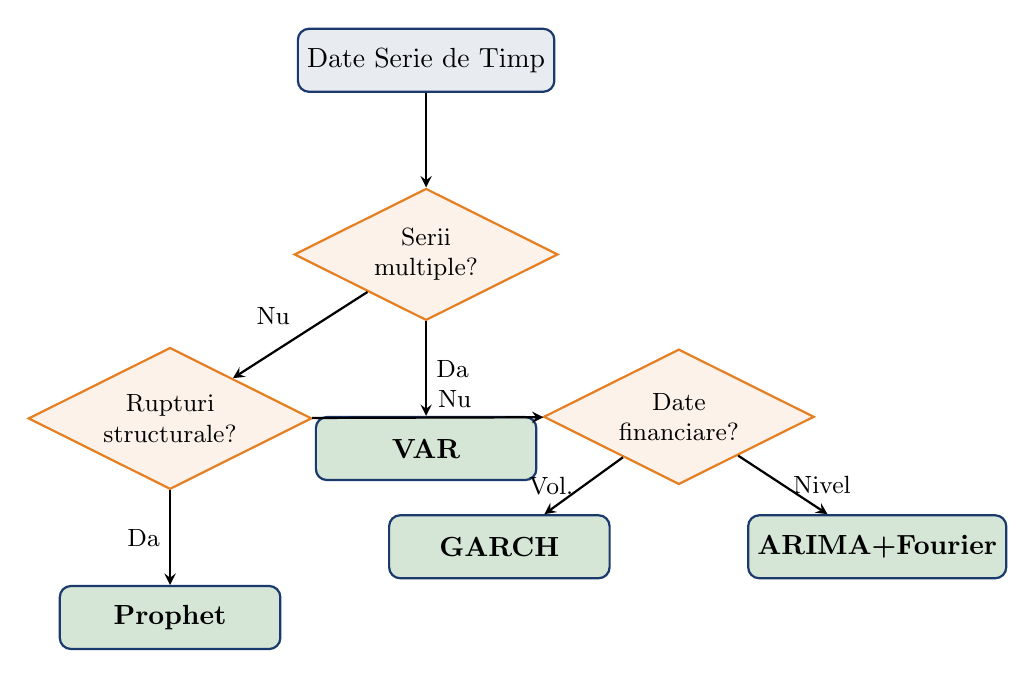
\begin{tikzpicture}[scale=1.0, transform shape,
        node distance=1.2cm,
        box/.style={rectangle, draw=MainBlue, thick, fill=MainBlue!10, rounded corners, minimum width=2.8cm, minimum height=0.8cm, align=center},
        decision/.style={diamond, draw=Orange, thick, fill=Orange!10, aspect=2, align=center, font=\small},
        arrow/.style={->, thick, >=stealth}
    ]
        \node[box] (start) {Date Serie de Timp};
        \node[decision, below=of start] (q1) {Serii\\multiple?};
        \node[decision, below left=1.2cm and 1.5cm of q1] (q2) {Rupturi\\structurale?};
        \node[decision, below right=1.2cm and 1.5cm of q1] (q3) {Date\\financiare?};
        \node[box, fill=Forest!20, below=of q1] (var) {\textbf{VAR}};
        \node[box, fill=Forest!20, below=of q2] (prophet) {\textbf{Prophet}};
        \node[box, fill=Forest!20, below left=0.8cm and 0cm of q3] (garch) {\textbf{GARCH}};
        \node[box, fill=Forest!20, below right=0.8cm and 0cm of q3] (arima) {\textbf{ARIMA+Fourier}};
        \draw[arrow] (start) -- (q1);
        \draw[arrow] (q1) -- node[right] {\small Da} (var);
        \draw[arrow] (q1) -- node[above left] {\small Nu} (q2);
        \draw[arrow] (q2) -- node[left] {\small Da} (prophet);
        \draw[arrow] (q2) -- node[above right] {\small Nu} (q3);
        \draw[arrow] (q3) -- node[left] {\small Vol.} (garch);
        \draw[arrow] (q3) -- node[right] {\small Nivel} (arima);
    \end{tikzpicture}
    \end{center}
\end{frame}

\begin{frame}{Sumar: Comparație Modele}
    \begin{columns}[T]
        \column{0.55\textwidth}
        \begin{center}
        \footnotesize
        \begin{tabular}{llll}
            \toprule
            \textbf{Caz} & \textbf{Provocare} & \textbf{Model} & \textbf{RMSE} \\
            \midrule
            Bitcoin & Volatilitate & GARCH & 2,15 \\
            Pete solare & Sezonalitate & Fourier & 31,10 \\
            Șomaj & Ruptură & SARIMA & 0,12 \\
            Economic & Multi-var & VAR & 1,53 \\
            \bottomrule
        \end{tabular}
        \end{center}

        \column{0.45\textwidth}
        \begin{center}
            \includegraphics[width=\textwidth]{../charts/model_comparison.pdf}
        \end{center}
    \end{columns}

    \vspace{0.2cm}

    \begin{exampleblock}{Principiu Cheie}
        \textbf{Potriviți modelul cu caracteristicile datelor.} Alegeți în funcție de natura problemei și proprietățile datelor.
    \end{exampleblock}
\end{frame}

\begin{frame}{Comparație Cuprinzătoare a Modelelor}
    \begin{center}
    \footnotesize
    \begin{tabular}{lcccc}
        \toprule
        \textbf{Caracteristică} & \textbf{GARCH} & \textbf{Fourier} & \textbf{Prophet} & \textbf{VAR} \\
        \midrule
        \textbf{Țintă} & Volatilitate & Nivel & Nivel & Multiple \\
        \textbf{Sezonalitate} & Nu & Da (lungă) & Da (multiplă) & Nu \\
        \textbf{Rupturi structurale} & Nu & Nu & Da & Nu \\
        \textbf{Serii multiple} & Nu & Nu & Nu & Da \\
        \textbf{Interpretabil} & Mediu & Ridicat & Ridicat & Ridicat \\
        \textbf{Parametri} & Puțini & $2K$ & Auto & Mulți \\
        \textbf{Date lipsă} & Nu & Nu & Da & Nu \\
        \midrule
        \textbf{Ideal pentru} & Finanțe & Cicluri & Business & Macro \\
        \bottomrule
    \end{tabular}
    \end{center}

    \vspace{0.3cm}

    \begin{columns}[T]
        \column{0.5\textwidth}
        \begin{block}{Rezultatele Noastre}
            \begin{itemize}
                \item GARCH: MAE=1,82 (volatilitate)
                \item Fourier: RMSE=31,10 (cicluri)
                \item SARIMA: RMSE=0,12 (rupturi)
                \item VAR: RMSE mediu=1,53 (multi)
            \end{itemize}
        \end{block}

        \column{0.5\textwidth}
        \begin{exampleblock}{Insight Cheie}
            Fiecare model excelează în domeniul său. Arta constă în alegerea modelului potrivit caracteristicilor datelor.
        \end{exampleblock}
    \end{columns}
\end{frame}

\begin{frame}{Bune Practici pentru Prognoză Aplicată}
    \begin{columns}[T]
        \column{0.5\textwidth}
        \begin{block}{Metodologie}
            \begin{enumerate}
                \item \textbf{Explorați} datele temeinic
                \item \textbf{Testați} staționaritatea
                \item \textbf{Împărțiți} train/validation/test
                \item \textbf{Comparați} modele pe validare
                \item \textbf{Raportați} metrici pe test
            \end{enumerate}
        \end{block}

        \vspace{0.2cm}

        \begin{alertblock}{Greșeli Frecvente}
            \begin{itemize}
                \item Privirea în datele de test
                \item Supraajustare pe setul de antrenament
                \item Ignorarea ipotezelor modelului
                \item Neraportarea incertitudinii
            \end{itemize}
        \end{alertblock}

        \column{0.5\textwidth}
        \begin{exampleblock}{Sfaturi Practice}
            \begin{itemize}
                \item Începeți simplu (random walk, naiv)
                \item Adăugați complexitate doar dacă e necesar
                \item Vizualizați prognoze vs. valori reale
                \item Verificați reziduurile pentru tipare
                \item Raportați intervale de încredere
            \end{itemize}
        \end{exampleblock}

        \vspace{0.2cm}

        \begin{block}{Amintiți-vă}
            ``Toate modelele sunt greșite, dar unele sunt utile.'' \\
            \hfill --- George E. P. Box
        \end{block}
    \end{columns}
\end{frame}

%=============================================================================
% CONCLUSION
%=============================================================================
\begin{frame}{Concluzii Cheie}
    \begin{enumerate}
        \item \textbf{Metodologie Riguroasă}
        \begin{itemize}
            \item Împărțirea train/validation/test previne supraajustarea
            \item Setul de test trebuie să rămână neatins până la evaluarea finală
        \end{itemize}

        \vspace{0.2cm}

        \item \textbf{Potriviți Modelul cu Datele}
        \begin{itemize}
            \item Volatilitate financiară $\succ$ GARCH
            \item Sezonalitate lungă $\succ$ Termeni Fourier
            \item Rupturi structurale $\succ$ Prophet
            \item Serii multiple $\succ$ VAR
        \end{itemize}

        \vspace{0.2cm}

        \item \textbf{Interpretați Rezultatele cu Grijă}
        \begin{itemize}
            \item Cauzalitate Granger $\neq$ cauzalitate adevărată
            \item Performanța out-of-sample contează cel mai mult
            \item Modelele mai simple funcționează adesea mai bine
        \end{itemize}
    \end{enumerate}
\end{frame}

%=============================================================================
% REFERENCES
%=============================================================================
\begin{frame}{Referințe}
    \footnotesize
    \begin{thebibliography}{99}
        \bibitem{box2015} Box, G.E.P., Jenkins, G.M., Reinsel, G.C., \& Ljung, G.M. (2015). \textit{Time Series Analysis: Forecasting and Control}. Ed. 5, Wiley.

        \bibitem{hamilton1994} Hamilton, J.D. (1994). \textit{Time Series Analysis}. Princeton University Press.

        \bibitem{tsay2010} Tsay, R.S. (2010). \textit{Analysis of Financial Time Series}. Ed. 3, Wiley.

        \bibitem{hyndman2021} Hyndman, R.J., \& Athanasopoulos, G. (2021). \textit{Forecasting: Principles and Practice}. Ed. 3, OTexts.

        \bibitem{taylor2018} Taylor, S.J., \& Letham, B. (2018). Forecasting at Scale. \textit{The American Statistician}, 72(1), 37-45.

        \bibitem{bollerslev1986} Bollerslev, T. (1986). Generalized Autoregressive Conditional Heteroskedasticity. \textit{Journal of Econometrics}, 31(3), 307-327.

        \bibitem{sims1980} Sims, C.A. (1980). Macroeconomics and Reality. \textit{Econometrica}, 48(1), 1-48.
    \end{thebibliography}
\end{frame}

%=============================================================================
% DATA SOURCES
%=============================================================================
\begin{frame}{Surse de Date}
    \begin{block}{Date Reale Folosite în Acest Capitol}
        \begin{itemize}
            \item \textbf{Bitcoin}: Yahoo Finance (BTC-USD), 2019--2025
            \item \textbf{Pete Solare}: Dataset Wolfer din Statsmodels, 1900--2008
            \item \textbf{Șomaj SUA}: Federal Reserve FRED (UNRATE), 2010--2025
            \item \textbf{Variabile Economice}: FRED (GDPC1, UNRATE, CPIAUCSL, FEDFUNDS), 2000--2025
        \end{itemize}
    \end{block}

    \vspace{0.3cm}

    \begin{exampleblock}{Reproductibilitate}
        Toate analizele pot fi reproduse folosind notebook-ul Jupyter însoțitor: \\
        \texttt{chapter10\_lecture\_notebook.ipynb}
    \end{exampleblock}
\end{frame}

%=============================================================================
% FINAL SLIDE
%=============================================================================
\begin{frame}[plain]
    \begin{tikzpicture}[remember picture, overlay]
        \fill[IDAred] (current page.north west) rectangle ([yshift=-0.15cm]current page.north east);
    \end{tikzpicture}

    \vfill
    \begin{center}
        {\Huge\textbf{\textcolor{MainBlue}{Mulțumesc}}}\\[0.5cm]
        {\Large\textcolor{MediumGray}{Întrebări?}}\\[1cm]
        {\large Prof. Daniel Traian Pele, PhD}\\[0.2cm]
        {\texttt{danpele@ase.ro}}\\[0.5cm]
        {\footnotesize Academia de Studii Economice din București}
    \end{center}
    \vfill

    \begin{tikzpicture}[remember picture, overlay]
        \fill[IDAred] (current page.south west) rectangle ([yshift=0.15cm]current page.south east);
    \end{tikzpicture}
\end{frame}

\end{document}
